\subsection*{Датчик - экспоненциальное распределение}
\addcontentsline{toc}{subsection}{Датчик - экспоненциальное распределение}

\textbf{Задание:}\\
Используя метод обратной функции, получить последовательность случайных чисел, распределённых экспоненциально с заданным параметром $\lambda$. Проанализировать полученную последовательность. Оценить математическое ожидание  и дисперсию, построить гистограмму.\\

\textbf{Решение:}\\
Плотность распределения экспоненциального закона:
\begin{ceqn}
	\begin{align*}
		f(x) =
		\begin{cases}
			\lambda e^{-\lambda \cdot x} \quad x \geq 0\\
			0 \hspace{1.55cm} x < 0
		\end{cases}
	\end{align*}
\end{ceqn}

Функция распределения экспоненциального закона:
\begin{ceqn}
	\begin{align*}
		F(x) =
		\begin{cases}
			1 - e^{-\lambda \cdot x} \quad x \geq 0\\
			0 \hspace{2.15cm} x < 0
		\end{cases}
	\end{align*}
\end{ceqn}

Получается, что обратная функция $F^{-1}(x)$ будет выглядеть следующим образом:
\begin{center}
	$x = \dfrac{-ln(1-y)}{\lambda} = -\dfrac{ln(y)}{\lambda}$
\end{center}
Если подставлять вместо $y$ случайные равномерно распределённые значения, то можно получать требуемые числа.

Таким образом, была реализована функция на языке программирования Python. (Рисунок \ref{fig:exp_inverse_function_method_code})
\begin{figure}[h]
	\centering 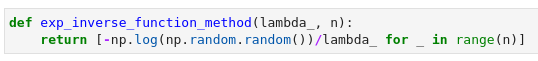
\includegraphics[scale=0.8]{exp_inverse_function_method_code}
	\caption{Реализация метода обратной функции для экспоненциального закона}
	\label{fig:exp_inverse_function_method_code}
\end{figure}

При $\lambda = 5$ и $n = 1000$ получается следующий результат. (Рисунок \ref{fig:exp_inverse_function_method_result})
\begin{figure}[h]
	\centering 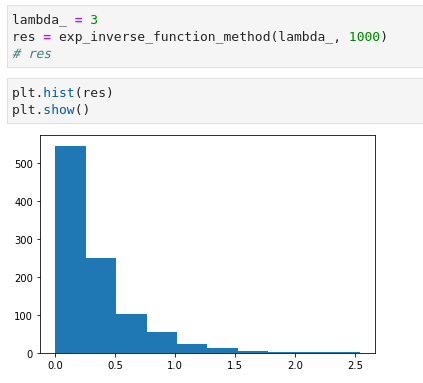
\includegraphics[scale=0.7]{exp_inverse_function_method_result}
	\caption{Результаты генерации случайных чисел методом обратной функции для экспоненциального закона}
	\label{fig:exp_inverse_function_method_result}
\end{figure}

Математическое ожидание экспоненциального распределения:
\begin{ceqn}
	\begin{align*}
		E = \dfrac{1}{\lambda}
	\end{align*}
\end{ceqn}
\newpage
Если рассчитывать математическое ожидание как среднее значение в выборке, то получается следующий результат. (Рисунок \ref{fig:exp_inverse_function_method_math})
\begin{figure}[h]
	\centering 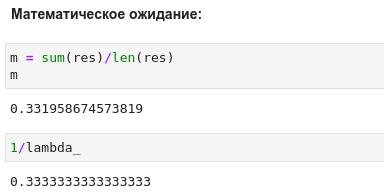
\includegraphics[scale=0.7]{exp_inverse_function_method_math}
	\caption{Теоретическое и расчётное значения математического ожидания ($\lambda = 3$)}
	\label{fig:exp_inverse_function_method_math}
\end{figure}

Можно заметить, что при $n = 1000$ значения получились достаточно близкими.\\
Дисперсия экспоненциального распределения:
\begin{ceqn}
	\begin{align*}
		D = \dfrac{1}{\lambda^2}
	\end{align*}
\end{ceqn}
Далее можно рассчитать дисперсию как среднее квадратное отклонение от среднего значения выборки. (Рисунок \ref{fig:exp_inverse_function_method_var})
\begin{figure}[h]
	\centering 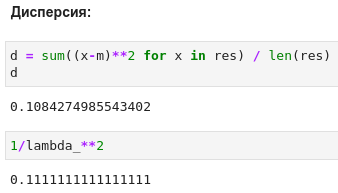
\includegraphics[scale=0.7]{exp_inverse_function_method_var}
	\caption{Теоретическое и расчётное значения дисперсии ($\lambda = 3$)}
	\label{fig:exp_inverse_function_method_var}
\end{figure}

Можно заметить, что при $n = 1000$ значения получились достаточно близкими.\\

Также стоит проверить гипотезу о том, что получившиеся значения распределены экспоненциально. Для этого воспользуемся критерием Колмогорова-Смирнова. (Рисунок \ref{fig:exp_inverse_function_method_test})
\begin{figure}[h]
	\centering 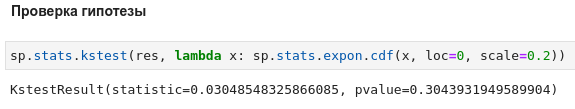
\includegraphics[scale=0.6]{exp_inverse_function_method_test}
	\caption{Результаты теста Колмогорова-Смирнова}
	\label{fig:exp_inverse_function_method_test}
\end{figure}

Значение \textit{p-value} > 0.05, значит мы принимаем гипотезу о том, что данная выборка имеет экспоненциальное распределение.